\chapter{Stand der Technik}

%%%%%%%%%%%%%%%%%%% Mechanik

\section{Kühlung} 

Bei dem Vorgang der Kühlung oder Abkühlung, wird einem System Wärme, oder thermische Energie entzogen. (Deshalb auch Entwärmung genannt)
Unter Kühlung versteht man die Übertragung von Wärme einer technischen Komponente, an die Umwelt. Das Phänomen der Kühlung wird und kann auch beabsichtigt hervorgerufen werden, um bestimmte temperaturabhängige Eigenschaften erreichen und erhalten, aber auch Systeme vor Überhitzung schützen zu können. 



\subsection{Thermodynamische Grundlagen}

Bei Feststoffen und Flüssigkeiten geht der Entzug von Wärme durch Wärmeübertragung entsprechend einem Temperaturgradienten vonstatten. Die wesentlichen Prozesse sind dabei Wärmeleitung und Wärmestrahlung, eingeschränkt auch die Konvektion. Diese Prozesse laufen spontan ab und deshalb, entsprechend der Gesetzen der Thermodynamik, einen Temperaturausgleich zur Folge haben. Diese Phänomen, kann für eine erwünschte Kühlung ausgenützt werden, jedoch ist hierfür viel Energie notwendig.  

Weil durch den Wärmeaustausch die Wärme nach Außen gelangt, hat dies eine Erhöhung der Temperatur, der Umgebung zur Folge. Dies bedeutet eine Umwandlung von Energieformen höherer Ordnung, in thermische Energie. Eine Kühlung im Sinne einer Reduzierung der thermischen Energie eines abgeschlossenen Systems ist daher nicht möglich, was sich in der Praxis zum Beispiel darin äußert, dass auch Kühlschränke letztlich die Temperatur (der Umgebung) erhöhen und nicht senken, wenn dies auch lokal der Fall sein mag.

Bei Festkörpern, ähnlich wie die elektrische Leitfähigkeit, gibt es auch bei der Wärmeleitung Einflussfaktoren. Diese sind hier Wärmeleitkoeffizient, Wärmeübergangskoeffizient und Wärmekapazität. Bei Flüssigkeiten spielt die Wärmeleitung und Wärmestrahlung ebenfalls eine Rolle, hinzu kommt jedoch die Konvektion als wesentlicher Prozess des Temperaturausgleichs. Bei Gasen dominiert die Konvektion.

\footnote{vgl. \cite{Kuehlung1} S.8-28}
\footnote{vgl. \cite{Kuehlung2}}

\newpage

\subsection{Technische Anwendung}

Kühlsysteme können nach dem verwendeten Wärmeträgermedium unterteilt werden. Die geläufigsten Arten der Kühlung sind:

\begin{itemize}
	\item Wasserkühlung und
	\item Luftkühlung.
	\item Ölkühlung z.  B. im Automotor und in Hydrauliksystemen (hydraulischen Antrieben) 
	\item Natriumkühlung in Kernkraftwerken
	\item Kühlung durch Peltier-Elemente Kühlung von Prozessoren
\end{itemize}

\subsection{Funktionsweise}

Die Kühlung verwendet diese in den Thermodynamischen Grundlagen genannten Phänomene und führt diese künstlich herbei. Diese basiert auf der Wärmeleitung, vom zu kühlenden Körper mit einem Kühlstoff, durch Gas oder Flüssigkeit und des Abtransports, also der Wärmeströmung. Um Platz zu sparen, werden in manchen Anwendungen, als Abtransport, Heatpipes verwendet. Bei Verbrennungs- und Elektromotoren werden oft6 Flüssigkeitskühlungen verwendet.



\subsection{Technische Kühlungsbeispiele}

\begin{itemize}
	\item Kühlsysteme von Kraftwerken und chemischen Prozessen
	\item Kühlung in der Klimatechnik
	\item Öl- und Ladeluftkühler im Turbodiesel-Motor
	\item Abgaskühlung in AGR-Systemen (zur Emissionsreduzierung (NOx))
	\item Wasserkühlung eines Automotors
	\item Luftkühlung eines Prozessors
	\item Kühlung für Steuerungen
\end{itemize}


\footnote{vgl. \cite{Kuehlung1} S.8-28}
\footnote{vgl. \cite{Kuehlung2}}

\newpage


\subsection{Wasserkühlung}  \label{Stand der Technik}

Bei einer Wasserkühlung (Flüssigkeitskühlung), wird logischerweise Wasser als primäres Kühlmittel verwendet. Für die Wasserkühlung gibt es sehr viele verschiedene Einsatzmöglichkeiten. Diese Art von Kühlung wird in Elektro- wie auch in Verbrennungsmotoren, Hochöfen, Stromrichtern, Kraftwerken, Computern und vielen weiteren Anwendungen verwendet.   

\subsubsection{Wasserkühlung bei elektronischen Geräten}

Röhren bestückte Endstufen werden seit fasst 100 Jahren mit einer Wasserkühlung gekühlt. Um Fehler von und deren Folgen, also Zerstörungen, zu vermeiden, wird bei dieser Art von Wasserkühlung kein normales Wasser verwendet, sondern nur destilliertes deionisiertes Wasser. Herkömmliches Wasser wäre bei dioesen großen Spannungen zu gefährlich. Bei einer Kühlung mit destillierten deionisierten Wasser, wird die Wärme durch einen Wärmeübertrager an einen zweiten Kühlkreislauf, welcher keine bestimmte Reinheit des Wassers besitzen muss, ab. Dieser Kreislauf ist von den hohen Spannungen so weit entfernt, dass keine Überschläge oder Kurzschlüsse mit dem Kühlwasser möglich sind. 

Eine weiter Kühlungsmethode verwendet die Siedekondensationskühlung, welche bei Hochleistungsröhren eingesetzt wird. Hier sind Dampferzeugung und Kondensation räumlich nicht voneinander getrennt. Die Kühlflüssigkeit, also das Kühlwasser fließt durch einen Kühlkanal, welcher mit Nuten versehen ist. Die Nuten sind hin zur Anodeninnenseite gerichtet.
In diesen Nuten entsteht durch die Erwärmung oder Erhitzung Wasserdampf. Der Wasserdampf gelangt nun in den Hauptkühlkanal, wo er durch Verwirbelung wieder kondensiert wird.

Dieser Vorgang geschieht bei Temperaturen von über 100°C und nützt zu gleich den Aggregatzustand flüssig zu gasförmig aus. Durch die hier benötigte Hitze für die Verdampfung, kann durch diese Kühlungsmethode auch bei kleinen Röhren große Wärmemengen abgeführt werden.

Neuere Modelle dieser Sender sind nicht mehr mit einer Wasserkühlung ausgestattet.

Auch in der Leistungselektronik wird eine Flüssigkeitskühlung mit Wasser verwendet. Beispiele für die Leistungselektronik sind Stromrichter für Hochspannungs-Gleichstrom-Übertragung oder auch 
Traktionsstromrichter in Schienenfahrzeugen.

\footnote{vgl. \cite{Wasserkuehlung}}
\newpage

\subsubsection{Wasserkühlung in Personal Computern}

Sehr oft sind mittlerweile auch Wasserkühlungen in PC-Systemen zu finden. Diese Methode ist um einiges leiser und effizienter um einzelne Komponenten zu kühlen, als die herkömmlichen Luftkühlungen mit Ventilatoren. Mit der Wasserkühlung wird meist der Hauptprozessor gekühlt. Neben dem Hauptprozessor, können noch Grafikkarten, Hauptplatinenchipsätze, Festplatten, Netzteile mit dem Transformator, Spannungswandler und RAM-Bausteine in die Wasserkühlung mit einbezogen werden.
Durch die Effizienz der Flüssigkeitskühlung mit Wasser und der immer weiter steigenden Leistungen, auch von Personalcomputern, ist um die Wasserkühlung bei Rechnern ein Markt entstanden.

Vorteile von einer Wasserkühlung sind unter anderem die schon erwähnte Effektivität der Kühlung der Hardware für Übertaktungsspielraum der CPU, durch die verbesserte Kühlung. Wie ebenfalls schon erwähnt funktioniert diese Kühlung sehr leise und beginnt nicht zu laut blasen, wenn eine große Rechenleistung vom PC verlangt wird. Bei der Wasserkühlung wird als Wärmeübertrager, ein Radiator, mit großen, langsam drehenden Lüftern oder ein passiver Radiatoren ohne Lüfter eingesetzt werden.
Noch nicht genannt, erhöht sich mit einer Wasserkühlung die Zuverlässigkeit und Lebensdauer der durch die Kühlung, gekühlten Bausteine. Durch die Verwendung der richtigen Pumpe kann die Methode der Wasserkühlung eine sehr stromsparende sein

Nachteile bringt diese Methode natürlich auch mit sich. Die Wasserkühlung, hat einen erheblich größeren Installationsaufwand und damit auch vergleichsweise hohe Kosten zur Folge. Mit den Genannten Problemen kommt auch noch die Wartung hinzu, weil nicht nur der Ventilator geputzt erden müssen.  Durch den Verzicht der Kühlung von einzelnen Komponenten, kann dies zur Überhitzung der selbigen führen. Mit hinzu kommt auch noch der erheblich größere Platzbedarf im Gehäuse. 

Weil destilliertes Wasser, verglichen mit anderen Kühlungsflüssigkeiten bei Zimmertemperatur, den größten Wärmeleitkoeffizienten besitzt, ist diese Flüssigkeit die erste Wahl bei einer Flüssigkeitskühlung.

\footnote{vgl. \cite{Wasserkuehlung}}
\newpage

\subsection{Luftkühlung} 

Elektronische Bauelemente der Leistungselektronik, Verbrennungsmotoren und Klimaanlagen werden bei der Luftkühlung, durch die an den Oberflächen vorbei strömende Luft gekühlt.
Die bei einer Luftkühlung benötigte Luftströmung kann durch verschiedene Arten erreicht werden. Unter andern durch Konvektion, Gebläse, also Ventilatoren, oder bei Fahrzeugen durch den Fahrtwind. 
Das Luftgekühlte Bauteil steht entweder so frei, dass es von Luft umströmt wird oder der Luftstrom wird mittels Kanäle um die Komponente geleitet. Oft sind freistehende Komponenten mit Kühlkörper aus einem Metall oder Kühlrippen als Wärmeübertrager versehen. Durch Rippen wird die Oberfläche vergrößert und dies hat einen größeren Wärmeabtransport zur Folge.

\subsubsection{Luftkühlung bei Personalcomputern}

Mit der Größe eines Prozessors, steigt auch die Wärmeentwicklung. In aktuellen PCs eingebaute leistungsstarke Mikrochips, erzeugen erhebliche Verlustwärme. Diese Wärme wird meist durch eine Luftkühlung abgeführt, um eine thermische Überlastung der Chips zu verhindern.

Um die Wärmeentwicklung zu verringern, wurde die Betriebsspannung der Bauteile reduziert, weil die gesamte Aufnahmeleistung in Wärme umgesetzt wird. Ebenfalls werden bei normalen Betrieb nicht benötigten Bauteilen, die Taktfrequenz verringert oder die Bauteile auch ganz abgeschaltet um weniger oder keine unnötige Energie zu verbrauchen oder unnötige Wärme zu erzeugen. Trotz dieser Methoden, reicht die Abfuhr der Wärme durch Strahlung und Konvektion nicht mehr aus.
Aus diesem Grund müssen Kühlkörper und Ventilatoren benutzt werden. Die Ventilatoren, sind am Rand des Gehäuses mit Luftkontakt nach Außen angebracht. Diese bewirken einen Luftstrom bei den zu kühlenden Komponenten und bläst die Warme Luft nach außen. Gleichzeitig wird kalte Luft von der anderen Seite angesaugt. Dies kann durch Luftlöcher erzwungen werden, die an einem kühltechnisch sinnvollen Platz gewählt worden sin, damit alle Bauteile, die eine Kühlung benötigen, umströmt werden.
Durch die mit gerippten Kühlkörpern vergrößerten Oberfläche der Bauteile ist die Kühlung ausreichend und ein zuverlässiger Betrieb ist möglich. 

In einem Rechner wird die CPU am stärksten gekühlt. Neben der CPU werden auch, wie schon in der Wasserkühlung erwähnt, Prozessoren von Grafikkarten und auch das Netzteil mit Transformator mit gekühlt. Bei einer Luftkühlung natürlich mit der Luft.



Weitere Anwendung:
\begin{itemize}
	\item HiFi-Verstärker 
	 Kunststoff
\end{itemize}

\footnote{vgl. \cite{Luftkuehlung1}}
\footnote{vgl. \cite{Luftkuehlung2}}
\newpage


\subsection{Aktive Kühlung} 

Bei einer aktiver Kühlung wird eine Kühlung durch eine Pumpe oder einem Lüfter künstlich erzwungen und wird eingesetzt, wenn die Abfuhr der Wärme durch Strahlung und Konvektion nicht mehr ausreicht.

\subsubsection{Aufbau}

Eine aktive Kühlung besteht meist aus den folgenden Komponenten:

\begin{itemize}
	\item Kühlmittel
		\begin{itemize}
        	\item Wasser
         	\item Luft
         	\item Öl
         	\item speziellen Kühlflüssigkeit
     	\end{itemize}
\end{itemize}

Das Kühlmittel sorgt oft auch für die Schmierung der Bauteile. 

\begin{itemize}
     \item Antreibende Komponente
     	\begin{itemize}
        	\item Lüfter
         	\item Pumpe
     	\end{itemize}	
\end{itemize}

Diese Komponenten erzwingen einen Kühlmittelstrom. 
Bei einem Lüfter wird die Luft zu einem Luftstrom gezwungen und umströmt das zu kühlende Bauteil. Bei einer Pumpe fließt das Kühlmittel nicht nur zum zu kühlenden Objekt, sondern ebenfalls durch den Radiator, welcher die Flüssigkeit auf Ausgangstemperatur herunter kühlt.



Funktionsprinzip einer Aktiven Kühlung entspricht beispielsweise der Wasserkühlung.

Mittels einer Pumpe wird das Kühlmedium (Wasser, Kühlmittel) durch einen Kühlkreislauf, der aus Schläuchen oder Bohrungen (Nuten) besteht durch gepumpt. Am anderen Ende der Zubringleitung befindet sich das Objekt, welches gekühlt werden soll und wird von der Kühlflüssigkeit umflossen. 
Das Kühlmittel nimmt die Wärme auf und transportiert sie ab. Bei der Rückleitung fließt das Wasser durch den Radiator, welcher die Temperatur des Wassers reduziert und eine Erhitzung der Pumpe verhindert. 
Der Radiator gibt die Wärme durch Ventilatoren oder bei einem passiven Radiator durch Strahlung an die Umgebung ab. Dafür ist aber immer ein Temperaturgefälle notwendig, weil sonst eine Abgabe nicht möglich ist. und je größer das Gefälle ist, desto mehr Wärme kann pro Zeit abgegeben werden.


\footnote{vgl. \cite{AktiveKuehlung}}

\subsection{Passive Kühlung} 

Die passive Kühlung ist im Grunde jede natürliche Abkühlung von Körpern. Hier wird das Phänomen der Wärmekonvektion verwendet. Diese Kühlung wird verwendet um die Erwärmung eines Motors, oder einer Maschine und elektrischen Geräten an die Umwelt abzugeben. Der Effekt für die Konvektion kann durch Kühlrippen verstärkt werden. Bei jeder aktiven Kühlung, sind also auch passive Kühlungen vorhanden, weil man die Wärme noch nicht "zwingen" kann von einem Köper an die Umgebung abzugeben. 

Eine passive Kühlung benützen zum Beispiel Kühlrippen oder Radiatoren. Diese Elemente bestehen aus Metall und geben die Wärme des wärmeren Mediums an das Kältere weiter. Um eine Beschleunigung zu erlangen, wird eine passive Kühlung mit eingesetzt.

\footnote{vgl. \cite{PassiveKuehlung}}

%%%%%%%%%%%%%%%%%%%%%%%%%%%%%%%%%%%%%%%%%%

\newpage

\section{Schutzarten Elektrischer Betriebsmittel} 

Die Schutzart eines Betriebsmittels gibt an, wie gut dieses geschützt ist vor:
\begin{itemize}
	\item Zugang von Personen zu gefährlichen Teilen innerhalb eines Gebäudes
	\item Eindringen von fremden Festkörpern
	\item Eindringen von Wasser
\end{itemize}
 
Die Angabe der Schutzart erfolgt in Form eines Kurzzeichens (IP-Code/ International-Protection-Code)
Dieser Schutz entspricht den Regeln von ÖVE/ÖNORM EN 60529 (und IEC)

Die erste Kennziffer, gibt den Schutz gegen Berührung von gefährlichen Teilen innerhalb des Gehäuses und den Schutz gegen das Eindringen von festen Fremdkörpern an.
Die zweite Kennziffer gibt den Schutz gegen Eindringen von Wasser an.

\begin{table}[H]
	\begin{tabular}{|c|c|c|c|l}
\cline{1-4}
		\textbf{Schutzart} & \textbf{Betriebsmittelschutz} & \textbf{Personenschutz}    & \textbf{Anwendung}             &  \\ \cline{1-4}
		IP6X               & staubgeschützt                & gegen eindringen von Draht & Deckelverschluss der Akkupacks &  \\ \cline{1-4}
		IPX7               & zeitweilig wasserdicht        & -                          & Gesamtes Akkupack              &  \\ \cline{1-4}
		IPX8               & dauerhaft wasserdicht         & -                          & Akkupack-Korpus                &  \\ \cline{1-4}
	\end{tabular}
	\caption{Auszug IP Schutzarten}
\end{table}

\footnote{vgl. \cite{IPSchutzarten} S.63,64}
\newpage

\section{Solid Edge}


\begin{figure} [H]
	\begin{center}
		
\includegraphics[scale=0.5]{figures/mechanik/Untitled.jpg}
			\caption{Solid Edge Logo}
			\label{fig:Solid Edge Logo}
	\end{center}
\end{figure}


Dank 1,5 jähriger Ausbildung in den ersten beiden Jahren in der HTBLuVA-Salzburg, konnte als Planungs- und Berechnungsprogramm, Solid Edge verwendet werden. 
Es wurden alle Teile des Motorrades in diesem Programm erstellt und geplant. Bei den Seitenplatten war noch eine Berechnung der Stabilität notwendig; um die Sicherheit prüfen zu können. 

\subsection{Erklärung}

Solid Edge ist ein 3D-Zeichenprogramm aus dem Hause Siemens. Auf einfachsten Wege, können virtuell Teile erstellt, auf Zeichenblättern für die Fertigung gedruckt und mit anderen Teilen zu Geräten miteinander verbunden werden. 

Mit der Funktion "DIN Metrisch Part" können Einzelteile erstellt und dimensioniert werden. In dieser Funktion sind einige Zeichenhilfen vorhanden, die einem das Zeichnen und planen erleichtern. Unter dem Abteilung "Volumenkörper" kann festgelegt werden, wie das Teil später einmal hergestellt werden soll. Beispielsweise wäre ein Rotationsausschnitt eine Fertigungsweise, einer Drehmaschine.


\begin{figure} [H]
	\begin{center}
		\includegraphics[scale=0.4]{figures/mechanik/Solid Edge_Volumenkörper.jpg}
			\caption{Solid Edge Volumenkörper}
			\label{fig:Solid Edge Volumenkörper}
	\end{center}
\end{figure}


Mit "Bemaßen" werden Maße des Formkörpers festgelegt.


\begin{figure} [H]
	\begin{center}
		\includegraphics[scale=0.4]{figures/mechanik/Solid Edge_BemaßenZeichn.jpg}
			\caption{Solid Edge Bemaßen}
			\label{fig:Solid Edge Bemaßen}
	\end{center}
\end{figure}


In der selben Funktion, lassen sich auch Berechnungen durchführen.
Unter der Registerkarte Simulationen, sind alle hierfür notwendigen Werkzeuge zu finden.
Mit "Strukturelle Lasten", können an den gewünschten Punkten, beliebige Arten und Größen von Kräften angelegt werden. 


\begin{figure} [H]
	\begin{center}
		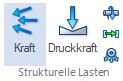
\includegraphics[scale=0.4]{figures/mechanik/Solid Edge_Strukturelle Lasten.jpg}
			\caption{Solid Edge Strukturelle Lasten}
			\label{fig:Solid Edge Strukturelle Lasten}
	\end{center}
\end{figure}


Der nächste Schritt besteht darin eine "Vernetzung" durchzuführen, um die Berechnung zu ermöglichen. Durch die Vernetzung, wird die Kontur des Bauteiles vernetzt, welche bei der Berechnung des Verhalten des Teiles auf die Kräfte, notwendig ist. 


\begin{figure} [H]
	\begin{center}
		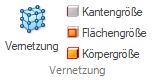
\includegraphics[scale=0.4]{figures/mechanik/Solid Edge_Vernetzung.jpg}
			\caption{Solid Edge Vernetzung}
			\label{fig:Solid Edge Vernetzung}
	\end{center}
\end{figure}


Mit "Berechnen", wird die Berechnung gestartet und das Ergebnis ausgegeben.
Im Ergebnis können die Verschiebung des Teiles, auftretende Spannungen und viele weitere Ergebnisse abgerufen und auch mit "Animation", animiert beobachtet und abgelesen werden. 


\begin{figure} [H]
	\begin{center}
		
\includegraphics[scale=0.4]{figures/mechanik/Solid Edge_Animation.jpg}
			\caption{Solid Edge Animation}
			\label{fig:Solid Edge Animation}
	\end{center}
\end{figure}


Die Funktion "DIN Metrische Zeichnung", kann das Bauteil in 2D Ansichten, für Zeichnungen umgewandelt werden, um das Bauteil fertigen lassen zu können. Die umgewandelten Ansichten können bemaßt und geschnitten werden, um ein bestmögliches Verständnis der Fertigungsabteilung zu versichern. Mit "Ansichtsassistent" kann das gewünschte Teil ausgewält unf umgewandelt werden.


\begin{figure} [H]
	\begin{center}
		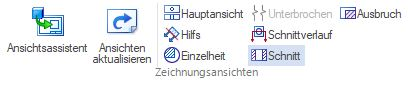
\includegraphics[scale=0.4]{figures/mechanik/Solid Edge_Zeichnungsansichten.jpg}
			\caption{Solid Edge Zeichnungsansichten}
			\label{fig:Solid Edge Zeichnungsansichten}
	\end{center}
\end{figure}


Mit der Funktion "DIM Metrische Baugruppe", können Einzelteile zu einem virtuellem Gerät zusammengebaut werden. Hier wird unter anderem ermöglicht Simulationen von Bewegungs- ,oder Getriebeabläufen zu erstellen. Durch die "Komponentenmontage" werden Beziehungen zwischen Teilen festgelegt und fixiert.

\begin{figure} [H]
	\begin{center}
		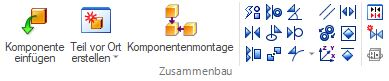
\includegraphics[scale=0.5]{figures/mechanik/Solid Edge_Zusammenbau.jpg}
			\caption{Solid Edge Zusammenbau}
			\label{fig:Solid Edge Zusammenbau}
	\end{center}
\end{figure}
\newpage

\section{Akkusysteme}
Verschiedene Speicher für elektrische Energie, die auf einer elektrochemischen Basis basieren, nennt man Batterien oder auch Akkumulatoren. Elektrochemische Speicher haben in den vergangenen Jahren immer mehr an Bedeutung gewonnen und werden auch in Zukunft immer öfter Gebrauch finden. Möglich wurde unsere heutige elektronische Mobilität erst mit der Erfindung der galvanischen Zelle. Seit dieser Erfindung,die mit Hilfe eines Stromkreises chemische Energie in elektrische Energie umzuwandeln, hat sich über die jahrzehntelange Weiterentwicklung der Batterie einiges getan. Die Einsatzmöglichkeiten von Akkumulatoren sind extrem vielfältig. Kleine Lithium-Ionen Akkus werden zum Beispiel als Knopfzellen in Smartphones verwendet. Jedoch können sie auch bis hin zu großen stationären Energiespeichern für erneuerbare Energien benutzt werden. Wie bereits vorher erwähnt, sind elektrische Energiespeicher ein wichtiger Bestandteil für den Erfolg der Elektromobilität geworden. Es gibt unzählig viele verschiedene Arten von Batterien, die sich im chemischen Aufbau, ihrer Form und natürlich in ihren Einsatzmöglichkeiten unterscheiden. Durch die äußerst besonderen chemischen Eigenschaften und die vielseitigen Anwendungsbereiche, hat sich der Lithium-Ionen Akku durchgesetzt.
\newpage

\section{Batteriearten}

\subsection{Bleiakkumulator}
Die ersten Versuche, einen auf Blei basierenden Akkumulator zu entwickeln, wurden am Anfang des 19. Jahrhunderts durchgeführt. Industriell wurde der Bleiakku interessant, als Forscher und Chemiker zusammen 1880 ein Verfahren entwickelten, bei dem der Bleiakkumulator bereits nach wenigen Ladezyklen, eine hohe Kapazität erreichte. Der erste technisch einsetzbare Bleiakkumulator wurde 1886 von Henri Tudor entwickelt. Dieser besitzt eine Zellspannung von ungefähr 2V (abhängig vom Ladezustand), was eine durchaus große Spannung für sogenannte "wässrige Syteme"  ist. Der Ausdruck "wässrige Systeme"  leitet sich von dem Elektrolyt ab. Bei Bleiakkumulatoren wird wässrige Schwefelsäure als Elektrolyt verwendet. Im entladenen Zusatnd bestehen beide Pole aus Blei(II)-sulfat (PbSO4). Weiters besteht die Kathode aus Blei und die Anode aus Bleioxid. Bleiakkumulatoren sollten keinesfalls tiefenentladen werden, da dies zu Schäden führt und den Akku unbrauchbar macht. Ein extrem großer Nachteil ist das Gewicht, da nur 30 bis 40Wh/kg erreicht werden können.
Diese Art von Akku zeichnet sich durch das kurzzeitige Zulassen hoher Ströme aus die zum Beispiel für Fahrzeug -bzw. Starterbatterien notwendig sind. Unter anderem sind 50 Prozent des Batteriemarkets von Bleiakkumulatoren belegt. Wie vorher bereits erwähnt werden diese oftmals in Autos, LKWs oder auch Motorräder verbaut.

\subsection{Nickel-Metallhybrid Akkumulatoren}
Die technischen Grundlagen des Nickel-Metallhybrid Akkumulator wurden von Stanford R. Ovshinsky und Masahiko Oshitani ab 1962 bis 1982 zur marktreifen Zelle entwickelt. Seit dem Jahr 2006 sind spezielle NiMH-Akkumulatoren auf dem Markt, die sich gegenüber herkömmlichen NiMH-Akkus durch eine deutlich reduzierte Selbstentladung auszeichnen. Die positive Elektrode eines Nickel-Metallhybrid Akkumulators(NiMH) besteht aus Nickel(II)-hydroxid wogegen sich die negative Elektrode aus einem Metallhybrid zusammensetzt. Als Elektorlyt verwendet dieser Akkumulator eine Wasserstoffspeicherlegierung aus Nickel und seltenen Erden. NiMH-Akkus erreichen bis zu 80Wh/kg. Sie sind vielfach in den üblichen Bauformen von Standardbatterien verbreitet und liefern pro Zelle eine Spannung von 1,2V. Oftmals werden sie als wiederaufladbare Alternative der gängigen Alkalibatterien in haushaltsüblichen Geräten eingesetzt. Ein großer Vorteil gegenüber den Nickel-Cadmium Batterien ist es, das der NiMH Akku nicht aus giftigen Cadmium besteht und er außerdem eine höher Energiedichte aufweist.
Der Anwendungsbereich von NiMH Akkumalatoren ist sehr vielfältig. Vorzugsweise kommen sie wie NiCd Akkus überall dort zur Anwendung, wo ein hoher Energiebedarf besteht und hohe Batteriekosten vermeiden werden sollten. Tyische Anwendungsbereich sind zum Beispiel Foto- Videogeräte, Elektroautos, Elektrowerkzeuge und noch viele mehr. NiMH Akkus werden außerdem oft als Energiespeicher für Notbeleutungsanlagen verwendet.
\newpage
\subsection{Nickel-Cadmium Akkumulatoren}
1899 wurde der Nickel-Cadmium Akku von dem Schweden W. Jungner entwickelt. NiCd Akkus zeichnen sich dadurch aus, dass sie einen eingebauten Ent- und Überladeschutz integriert haben. Das hat zur Folge, dass man keine aufwendige elektronische Beschaltung durchführen muss. Als Material für die Kathode dieses Akkus verwendet man Nickeloxidhydroxid. Die Anode dagegen besteht aus dem giftigen Material Cadmium, welches jedoch eine äußerst hohe spezifische Ladung (478Ah/kg) besitzt. Bei Nickel-Cadmium Akkumulatoren besteht das Elektorlyt aus Kalilauge. Die typische Nennspannung ist exakt die selbe wie bei NiMH Akkus, 1,2V. Aus dieser Zellenspannung ergibt sich eine spezifische Energie von ungefähr 60Wh/kg. Eine Eigenschaft die man bei anderen Technologien nur selten antrifft ist das hervorragende Tieftemperaturverhalten von NiCd Akkus. Selbst bei einer Temperatur von -40°C ist eine Inbetriebnahme noch möglich. Im Jahr 2004 wurde jedoch die Verwendung von Nickel-Cadmium Akkus wegen dem giftigen Material auf medizinische und sicherheitrelevante Bereiche begrenzt. Diese Akkumulatoren sind in 2 verschiedenen Bauformen verfügbar, die sich durch die unterschiedlichen Anwendungsbereiche unterscheiden. Die offene Bauweise wird meist für Starterbatterien für Verbrennungsmotoren und Traktionsbatterien für Elektrofahrzeuge verwendet. Bei der anderen Bauweise, werden die Zellen gasdicht verschlossen. Oftmals werden sich für zentrale Stromversorgungssysteme für Notbeleuchtung verwendet.
\newpage

\subsection{Lithium-Ionen Batterie}
\subsubsection{Geschichte}
Schon bereits in dem Jahr 1970 wurde von Jürgen Otto Besenhard und anderen das grundlegende Funktionsprinzip der Alkalimetallionen-Interkalation in Kohlenstoff-Elektroden sowie auch in oxidischen Elektroden erforscht und veröffentlicht. Ebenfalls wurde dabei die Anwendung in Lithium Batterien untersucht auch wenn zu der Zeit die praktische Anwendbarkeit als Elektroden für Lithium Batterien noch nicht erkannt wurde. Der erste auf dem Markt erhältliche Lithium-Ionen Akkumulator wurde von Sony im Jahr 1991 angeboten. Dieser Lithium-Cobaltdioxid Akku wurde in einer Videokamera verbaut. Die Batterie, die eine Spannung von 7,2V aufweiste, bestand aus zwei seriell verschalteten Zellen und weiste etwa eine Kapazität von 1200mAh auf. Sogar bis heute wird diese Bauform von Akkumulatoren mit Kapazitäten
bis zu 6900mAh angeboten und in äußerst vielen Geräten eingesetzt. Drei Physiker bzw. Chemiker (Whittingham, Goodenough und Yoshino) erhielten 2019 sogar den Nobelpreis für Chemie, für die Entwicklung der Lithium-Ionen Batterie.
Forscher einer Universität fanden im Jahr 2020 heraus, dass durch die Zugabe von dem Element Kalium die Lithium Akkumulatoren langlebiger und sicherer werden. Außderdem verhindert das Kalium in dem Akku unerwünschte chemische Nebenreaktionen.
\subsubsection{Allgemeines}
Es gibt zahlreiche verschiedene Bauformen von Lithium-Ionen Akkumulatoren. Diese Batterien unterscheiden sich nicht nur in ihrer Größe und der Bauform, sondern auch in der chemischen Zusammensetzung ihrer Komponenten und haben unter anderem auch verschiedene Spannungsbereiche. Kenndaten wie Zellenspannung, Lade- und Entladeschlussspannung, Temperaturempfindlichkeit und der maximal zulässige Lade- oder Entladestrom variieren bauartbedingt und sind wesentlich vom eingesetzten Elektrodenmaterial und den Elektorlyten abhängig. Eine Eigenschaft die alle Lithium-Ionen Akkumulatoren gemeinsamen haben ist, dass sie gasdicht versiegelt sein müssen und außerdem lageunabhängig betrieben werden können. Die spezifische Energiedichte liegt ungefähr in der Größenordnung von 150Wh/kg und weist eine Energiedichte von 400Wh/l auf. Durch diese Eigenschaften findet diese Art von Batterie besonderen Einsatz in der mobilen Branche als elektrischer Energiespeicher. Ein weiteres wichtiges Merkmal aller Lithium-Ionen Akkumulatoren ist, dass sie Überladungen nicht verkraften können. Wenn man mehrere Zellen zum Beispiel in Reihe schaltet, um eine höhere elektrische Spannung zu erzielen, müssen zum Ausgleichen der Toleranzen in der Kapazität zwischen den Zellen meistens zusätzlich ein Batteriemanagementsystem (BMS) und ein Balancer vorgesehen werden.  
\newpage

\subsubsection{Prinzip der Lithium-Ionen Batterie}
Ein Lithium-Ionen Akkumulator erzeugt durch die Verschiebung von Lithium-Ionen eine elektromotorische Kraft.
Beim Ladevorgang wandern positiv geladene Lithium-Ionen durch einen Elektrolyten hindurch von der positiven Elektrode zur negativen, während der Ladestrom die Elektronen über den äußeren Stromkreis liefert. Eine negative Elektrode aus Lithium-Metall ist elektrochemisch optimal, für einen Akku aber ungeeignet. Da sich die Elektrode beim Entladevorgang genauso wie bei einer Lithium-Batterie auflöst, besteht beim Ladevorgang keine Möglichkeit mehr, ihre Geometrie zu rekonstruieren.

\textbf{Aufbau:}

Die negative Elektrode eines gänigen Lithium-Ionen Akkus besteht meist aus Graphit. Die positive Elektrode hingegen enthält meist Lithium-Metalloxide in Schichtstruktur wie Lithiumcobaltoxid (LiCoO2). Der Lithium-Ionen Akkumulator muss wasserdicht sein, da es sont zu einer Nebenreaktion zwischen dem Wasser (H2O) mit dem Leitsalz (LiPF6) zu Flusssäure (HF) reagieren kann. Das am häufigsten verwendete Elektrolyt in Lithium-Ionen Akkumulatoren besteht aus einer Mischung zwischen wasserfreien Lösungsmitteln (Ethylencarbonat, Propylencarbonat) mit Alkylcarbonaten/Äthern (Dimethylcarbonat, Diethylcarbonat) und natürlich mit Lithiumsalzen.

Beim Aufladen der Lithium-Ionen Akkus, d.h. anlegen einer äußeren Potenzials, fließen Lithium-Ionen zwischen die Graphitebenen (nC). Zusammen mit dem Kohlenstoff bilden diese Ionen eine Interkalationsverbindung (LixnC). 
Anders als beim Aufladen, wandern die Lithium-Ionen beim Entladen wieder in das Metalloxid und die Elektronen der Batterie können über einen äußeren Stromkreis wieder zur positiven Elektrode fließen. 
Ausschlaggebend für diese Interkalationsverbindung ist die Ausbildung einer schützenden Deckschicht auf der neagtiven Elektrode. Für die Lithium-Ionen ist diese Schicht durchlässig, jedoch die Lösungsmittelmoleküle können diese Deckschicht nicht durchdringen. Es kann passieren, dass diese Deckschicht nicht genügend ausgebildet worden ist. Das hat zur Folge, dass die Lithium-Ionen mit den Lösungsmittelmolekühlen interkalieren, wodurch die Graphitelektrode stark beschädigt, oder sogar zerstört wird.

\textbf{Reaktionsgleichungen:}
\begin{itemize}
	\item \textbf{Negative Elektrode (Entladung):} \medskip\\
	LiCn  -->  nC + xLi+ + xe-

	\item \textbf{Positive Elektrode (Entladung):}\medskip\\
	LiMn2O4 + xLi+ + xe-  -->  LiMn2O4

	\item \textbf{Redox Gleichung:}\medskip\\
	LiMn2O4 + LiCn  -->  LiMn2O4 + nC
\end{itemize}

\begin{figure}[H]
	\begin{center}
		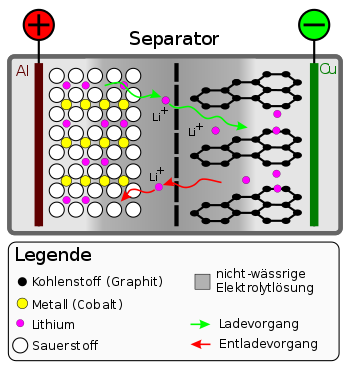
\includegraphics[scale=0.5]{figures/Akku/350px-Li-Ion-Zelle_(CoO2-Carbon,_Schema).svg.png}
		\caption{Grundaufbau einer Lithium-Ionen Zelle}
	\end{center}
\end{figure}
\newpage

\subsubsection{Lagerung und Sicherheithinweise}
Auch wenn Lithium nur als Li-Verbindungen in Lithium-Ionen Akkumualtoren vorhanden sind, sind die Komponenten eines solchen Akkus extrem leicht entzündbar, da Lithium ein hochreaktives Metall ist. Beim Überladen sind Ausgleichsreaktionen (z.B. die Zersetzung von Wasser), bei Lithium-Ionen Akkus nicht möglich, wie bei anderen Akkumualtoren dies der Fall ist. Schutzschaltungen die intern verbaut sein sollten, müssen eine solche Verpufferung verhindern. Anderfalls wird sonst die Funktionsfähigkeit des Akkus zerstört und er wird unbrauchbar. 
Jedoch kann es nicht nur zu inneren Beschädigungen kommen. Im Falle von inneren Kurzschlüssen, kann es passieren, dass mechanische Beschädigungen entstehen. Der hohe Kurzschlussstrom lässt zum Beispiel das Gehäuse schmelzen oder sogar in Flammen aufgehen. Es kann auch passieren, dass man den Defekt nicht unmittelbar erkennen kann. Doch kurze Zeit später kann es bereits zum Ausbruch eines Feuers kommen.

\textbf{Lagerung:}

Im Idealfall, sollten Lithium Ionen Akkus bei einem Ladezustand zwischen 40 - 60 Prozent kühl aufbewahrt und gelagert werden.


\textbf{Sicherheitshinweise:}

\begin{itemize}
	\item{Es ist wichtig, dass Lithium-Ionen Akkus nur mit passenden Ladegeräten aufgeladen werden. Schnell-Ladegeräte für Lithium Akkumulatoren können beispielweise eingesetzt werden. Man muss darauf achten, dass sie immer unter Aufsicht und möglichst nicht in der Nähe von brennbaren Materialien benutzt werden.} \medskip\\

	\item {Lithium-Ionen Akkus sind zwar hermetisch gekapselt, dennoch sollten sie unter keinen Umständen in Wasser getaucht werden. Besonders defekte und  vollgelade Lithium-Zellen reagieren meist heftig mit Wasser.}\medskip\\
	
	\item {Lithium-Ionen Akkumulatoren sind mechanisch sehr empfindlich. Durch einen internen Kurzschluss und einem Kontakt mit Luft können sie sich schnell entzünden.}\medskip\\
	
	\item {Eine Lithium-Ionen Zelle die in Flammen steht, wenn möglich mit Sand und nicht mit Wasser löschen, da dies zu einer heftigen Reaktion führen kann.}\medskip\\
	
	\item {Lithium-Zellen sollten niemals über 4,2V geladen und nicht unter 2,5V pro Zelle entladen werden. Außerdem dürfen Zellen niemals kurzgeschlossen werden. Bei einem Ladvorgang ist auf eine gute Wärmeabfuhr zu achten (nicht in die Sonne legen).}\medskip\\
	
	\item {Mehrere Lithium-Zellen sollten nur dann gleichzeitig geladen werden, wenn eine Schutzschaltung vorhanden ist.}\medskip\\
	
	\item {Die Elektorlytflüssigkeit ist brennbar. Sollte aus einer Zelle Elektrolytflüssigkeit austreten, diese am besten sofort ordnungsgerecht entsorgen.}\medskip\\
	
	\item {Man sollte versuchen die Lithium-Zellen bei einer Restkapazität von 20 Prozent nachzuladen.}\medskip\\

\end{itemize}
\newpage

\subsubsection{Anwendungbereiche von Lithium-Ionen Akkumulatoren}
Lithium-Ionen Akkus versorgten anfangs hauptsächlich tragbare Geräte mit hohem Energiebedarf, für die herkömmliche Nickel-Cadmium- oder Nickel-Metallhydrid Akkus zu schwer oder zu groß waren, beispielsweise Mobiltelefone, Tablets, Digitalkameras, Camcorder, Notebooks, Handheld-Konsolen oder Taschenlampen. In der heutigen Zeit sind Lithium-Ionen Akkumulatoren fast in allen denkbaren Bereichen aufzufinden. In der Elektromobiliätsbranche dienen sie oftmals als Energiespeicher für Elektroautos, moderne elektronisch betriebene Rollstühle und auch für Hybridfahrzeuge. Auch im Modellbau haben sie schon früh Verwendung gefunden. Dadurch, dass Lithium Akkus ein deutlich geringeres Gewicht als andere Batteriearten aufweisen, sind sie in Verbindung mit bürstenlosen Gleichstrommotoren und den entsprechenden Reglern, gut als Antriebseinheit im Flugmodellbau geeignet. Scho seit Anfang des 21. Jahrhunderts, gibt es Lithium-Ionen Akkus auch in Elektrowerkzeugen wie zum Beispiel Akkuschraubern. Auch im Flugbetrieb haben diese Batterien Verwendung gefunden. In der Boeing 787 werden ebenfalls Lithium-Kobaltoxid-Akkus (LiCoO2) verwendet. Zum Großen Teil werden Lithium-Ionen-Batterie-Systeme auch in Batterie-Speicherkraftwerken und Solarbatterien eingesetzt.
\newpage


\subsection{Batteriemanagementsystem}
\label{Batteriemanagementsystem}
Batteriemanagementsysteme (BMS) sind elektronische Regelschaltungen, die Akkumulatoren oder Akkupacks auf Ladung und Entladung überwachen und ebenfalls regeln. Die Batteriekennwerte die man überwachen kann bzw. möchte, hängen oftmals von dem Projekt ab. Zu den häufigsten Batteriekennwerten gehören die Erkennung des Batterietyps, die Batteriespannung, die Spannung sowie die Temperatur einzelner Batteriezellen, die Akkukapazität, der Ladzusatnd, die Restbetriebszeit, die Stromentnahme und einige Kennwerte mehr. Die Hauptaufgabe von BMS-Systemen besteht darin, sicherzustellen, dass die Restenergie in einer Zelle optimal genutzt wird. Um keine Beschädigungen an Zellen zu bekommen, schützt das Batteriemanagementsystem die Batterien vor Tiefenentladung, vor Überspannung, vor zu schneller Ladung (begrenzen des Ladestroms) und ebenfalls vor einem zu hohen Entladestrom. Bei Akkupacks, d.h. Akkumulatoren mit mehreren Zellen, sorgt das Batteriemanagementsystem außerdem für ein sogenanntes Balancing, das sich darin ausdrückt, dass die verschiedenen Batteriezellen gleiche Ladezustände und Entladezustände haben.

\begin{figure}[H]
	\begin{center}
		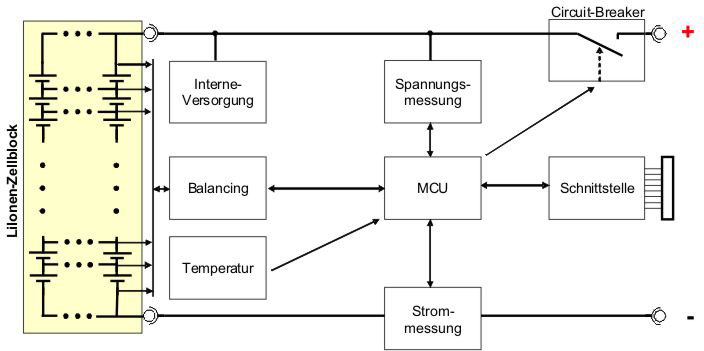
\includegraphics[scale=0.5]{figures/Akku/bms-1schaltunggrund.jpg}
		\caption{Grundschaltung eines Batteriemanagementsystems}
	\end{center}
\end{figure}

Grundsätzlich setzt sich ein vollständiges Batteriemanagementsystem aus folgenden Komponenten zusammen:
\begin{itemize}
	\item \textbf{Cell Supervising Circuit(CSC):} \medskip\\
	Die Aufgabe des CSC besteht darin die Zellen auf Spannung und 			Temperatur zu überwachen.

	\item \textbf{Kontrolleinheit:}\medskip\\
	Die Kontrolleinheit berechnet die State of Charge (SOC), die State 	of Health (SOH) und überprüft auch die Funktionalität der 				Batterien (State of Function). Außerdem wird von der 					Kontrolleinheit auch der Ladeausgleich gesteuert und kommuniziert 		über eine Serielle Schnittstelle mit einem Prozessor. 

	\item \textbf{Circuit Breaker:}\medskip\\
	Der Circuit Breaker trennt im Fehlerfall die Batterie von der 		Last. Dies erfolgt mithilfe eines HS-Kontaktors.
	
	\item \textbf{Strommessvorrichtung:}\medskip\\
	Diese Komponente ist für die Messung des Stromes zuständig.
	
	\item \textbf{Temperaturüberwachung:}\medskip\\
	Diese Komponente überprüft, ob sich die Batterien oder die 				Akkupacks in einem zulässigen Temperaturbereich befinden.
\end{itemize}
\newpage

\subsubsection{Komponenten eines BMS}

\textbf{Cell Supervising Circuit (CSC):}
Die erste Komponente eines Batteriemanagementsystem ist für die Spannungs- und Temperaturüberwachung der einzelnen Zellen zuständig und wird als Cell Supervising Circuit (CSC) bezeichnet. Ein Akkusystem besteht immer aus mindestens 2 einzelnen Zellen, oftmals jedoch aus mehreren. Deswegen ist die Spannungs- und Temperaturüberwachung jeder einzelnen Zelle nicht möglich. Es kommt  durchaus vor, dass mehrere einzelne Zellen zu sogenannten Akkupacks zusammengeschraubt oder zusammengeschweißt werden. Man hat dann wiederrum die Möglichkeit, jedes Akkupack für sich mithilfe eines CSC zu überwachen.

\textbf{Kontrolleinheit:}
Die nächste Komponente wird auch als Kontrolleinheit bezeichnet. Die Aufgabe dieser Komponente liegt darin, die SOC (State of Charge) und auch die SOH (State of Health) zu berechnen. Außerdem steuert die Kontrolleinheit auch den Ladeausgleich der einzelnen Zellen oder der Akkupacks. Diese Komponente übernimmt auch die Kommunikation des Batteriemanagementsystems mit anderen angeschlossenen Einheiten. Diese Kommunikation erfolgt über eine serielle Schnittstelle wie den I2C-Bus oder dem CAN-Bus. Die Werte (SOC und SOH) und auch die SOF (State of Function) werden dann an einen Prozessor übermittel auf dem die BMS-Software läuft und außerdem der SOC-Algorithmus implementiert ist. Die Kontrolleinheit ist fähig sich selbst in einen Ruhezustand zu versetzen um den eigenen Stromverbauch um ein Minimum zu reduzieren.

\begin{itemize}
	\item \textbf{State of Health (SOH):} \medskip\\
	Beschreibt den aktuellen Alterungszustand der Batterie. Ein Kriterium dafür ist, welche Ladungsmengen die Zellen noch aufnehmen. Je älter die Akkumulatoren werden, desto weniger Aufnahmevermögen haben sie.

\item \textbf{State of Charge (SOC):} \medskip\\
	Beschreibt den momentanen Ladezustand der Batterie. Außerdem gibt er Auskunft darüber, wie viel beziehungsweise wie lange die Batterie noch Energie bereitstellt. Beim Aufladen der Akkus gibt es an, wie viel Energie er noch aufnehmen kann.

\item \textbf{State of Function (SOF):} \medskip\\
	Gibt die Funktionalität der Batterie an. State of Function beschreibt die Leistungsfähigkeit der Batterie. Also wie viel kW der Energiespeicher dem Motor zum Beispiel bereitstellen kann. Die Leistungsfähigkeit lässt mit zunehmendem Batteriealter nach.
\end{itemize}

\textbf{Circuit-Breaker:}
Tritt ein Fehler bei einer einzelnen Zelle oder auch einem ganzen Akkupack auf, wird diese Batterie mithilfe eines HS-Kontaktors (Circuit-Breaker) von der Last getrennt. Dies schützt den Akkumulator. Dieser Kontaktor übernimmt außerdem noch die Trennung eines Akkumulatoren im Ruhezustand. Fehler die durch Trennen der Last beseitig werden können sind zum Beispiel Kurzschlüsse oder auch Übertemperatur. Für den Kurzschlussfall sind meisten auch noch Schmelzsicherungen (eine Art Sollbruchstelle im Stromkreis; die Wärmewirkung des Stromes wird ausgenutzt) verbaut die verhindern, dass Leitungen oder auch das Gehäuse in Flammen aufgehen.

\textbf{Strommessvorrichtung:}
Diese Komponete ist wie der Name schon beschreibt, für die Messung des Stromes zuständig. Oftmals werden dazu zwei voneinander unabhängige Systeme verwendet. Um den Strom messen zu können, wird ein Messsensor verwendet. Dies ist meist ein einfacher Widerstand. Bei der zweiten Methode wird der Strom über das elektromagnetische Feld gemessen.

\textbf{Temperaturüberwachung:}
Die letzte Komponente, die benötigt wird, um das Batteriemanagementsystem zu vervollständigen, ist für den Temperaturausgleich zuständig. Das heißt, es wird überwacht ob sich der Akkumulator in einem zulässigen Temperaturbereich findet. Sollte das nicht der Fall sein, können innere sowie auch äußere Schäden an der Batterie entstehen. Außerdem wirkt sich die Temperatur auf die Lebensdauer der Akkus auf.
\newpage

\subsubsection{Battery-Balancing}
\label{Battery-Balancing}
Der Ausdruck Balancing bezogen auf Akkumulatoren bedeutet so viel wie Ladeausgleich. Ohne Battery-Balancing bestimmt in einem Mehrzellen-Akku immer die schwächste Zelle darüber, welche Kapazität oder Spannung das Gesamtsystem aufweist. Das ergibt sich daraus, da sich jede Zelle minimal von einer anderen Zelle, durch ihre chemischen Struktur, unterscheidet. Einzelne Batteriezellen können auch unterschiedlich altern und deswegen kann man nie sicherstellen, dass jede Zelle exakt die identische Kapazität aufweist. Manche Zellen laden etwas schneller oder langsamer als andere. Wiederrum andere Batterien entladen sich etwas zügiger oder eben auch langsamer. In der Regel gibt es zwei verschiedene Arten von Battery-Balancing.
\begin{itemize}
\item \textbf{Passives Battery-Balancing} \medskip\\
\item \textbf{Aktives Battery-Balancing} \medskip\\
\end{itemize}


\textbf{Akkupacks:}

Muss noch zitiert werden: Cluster oder Akkupacks bestehen zur Erhöhung der Nennspannung in der Regel aus mehreren in Reihe geschalteten Einzelzellen oder Zellblöcken. Fertigungs- und alterungsbedingt gibt es hierbei Schwankungen in der Kapazität, im Innenwiderstand und weiteren Parametern dieser Zellen. Die schwächste Zelle ist dabei bestimmend, wie viel geladen oder entladen werden darf. Im praktischen Einsatz von mehrzelligen in Reihe verschalteten Akkus führt dieser Umstand dazu, dass die Zellen in Reihe unterschiedlich geladen und entladen werden.

Es kommt dann im Verbund zu kritischer Tiefentladung oder bei der Ladung zu einer Überladung und Überschreiten der Ladeschlussspannung einzelner Zellen. Je nach Akkutyp kann es dabei zu einer irreversiblen Schädigung einzelner Zellen kommen. Die Folge: das gesamte Akkupack verliert an Kapazität. (Ende des Zitates)
Um das zu verhindern, spielen im Batteriemanagementsystem die Balancer eine wichtige Rolle. Beim Battery-Balancing gibt es zwei verschiedene Arten. 
\begin{itemize}
\item \textbf{Passives Battery-Balancing} \medskip\\
\item \textbf{Aktives Battery-Balancing} \medskip\\
\end{itemize}

\newpage

\section{Synchronmaschine mit Dauermagneterregung}
\subsection{Allgemeines}
Die permanenterregte Synchronmaschine benötigt keine zusätzlichen Komponenten für die Einspeisung des Erregersystems. Neben dem Wegfall der Schleifringe bzw. des Kommutators hat die PSM noch weitere Vorteile:
\\[5mm]
\begin{itemize}
	\item Aufgrund der Erregung mit Permanentmagneten ist die Einspeisung einer flussbildenden Blindstromkomponente, wie bei der Asynchronmaschine bekannt ist, nicht notwendig. Somit ist der einzuspeisende Strom und damit der Energieverbrauch für vergleichbare Maschinen kleiner\footnote{vgl. \cite{Dissertation}, S. 15ff.}. \\[3mm]
	\item Weiteres erlauben die fehlende Läufernutung und die hohe Remanenzflussdichte der Dauermagneten höhere Luftspaltflussdichten, dadurch lassen sich auch höhere Leistunsdaten realisieren. \\[3mm]
\end{itemize}

Verglichen mit Asynchronmaschinen haben permanenterregte Synchronmotoren also eine mindestens doppelt so große Bemessungsleistung bei gleicher Baugröße, zudem besitzen sie ebenfalls weniger Gesamtverluste. Die PSM müssen jedoch anwendungsspezifischer ausgelegt werden, denn es entfallen alle Einflussmöglichkeiten auf die Betriebsdaten, speziell auf Betrag und Phasenlage des Ständerstroms, die sonst durch die Änderung des Feldes über den Erregerstrom gegeben sind.

\subsection{Aufbau}
Um eine gute Ausnutzung des Bauvolumens realisieren zu können, wird der Ständer meist mit einer sechspoligen Drehstromwicklung ausgeführt. Der Läufer ist dabei wie in folgender Abbildung beschrieben mit Dauermagneten ausgeführt. Große Aussparungen im Läuferblech (2) reduzieren das Trägheitsmoment und führen zu besseren dynamischen Eigenschaften\footnote{vgl. \cite{Fischer}, S. 348ff; S. 405}.
\\[3mm]
\begin{figure}[H]
	\begin{center}
		\includegraphics[scale=0.7]{figures/antrieb/Läufer_Synchronmaschine.jpg}
		\caption{Läufer einer dauermagneterregten Synchronmaschine\cite{Fischer}}
	\end{center}
\end{figure}

\subsection{Funktionsweise}
Im Motorbetrieb wird an die Klemmen der Ständerwicklungen ein Drehstrom angelegt und dadurch ein sinusförmiges Drehfeld erzeugt. Da sich ungleiche magnetische Pole anziehen, wird der Rotor mit seinem zugehörigen Magnetfeld synchron mit dem angelegten Drehfeld mitbewegt. Im Leerlauf stehen sich also der Norpol des Stator-Drehfelds und der Südpol des permanenterregten Rotor-Magnetfelds exakt gegenüber, die Drehzahl des Läufers ist also synchron mit der Drehzahl des angelegten Drehfelds. Bei bremsender Last eilt das Magnetfeld des Permanentmagneten dem Stator-Drehfeld um den Polradwinkel nach. Die Größe des Winkels stellt sich also abhängig von der Stärke des Lastdrehmoments ein. Dies kann jedoch nur bis zum sogenannten Kippmoment (Polradwinkel $\vartheta = 90^\circ$) gesteigert werden. Übersteigt das Drehmoment der Last das Kippmoment, so spricht man vom \glqq Abreißen\grqq{} der magnetischen Felder und die Synchronmaschine bleibt stehen. Das selbe gilt für den Generatorbetrieb, hier eilt aber das Drehfeld des Rotors vor. Bei Frequenzumrichterspeisung mit Feldorientierung kann jedoch dauerhaft mit $\vartheta$ = +/- $90^\circ$ gefahren werden, man spricht von sogenannter Querstromspeisung, der Zusammenhang zwischen (Läufer)-Feld und (Ständer)-Strom entspricht dann jenem der fremderregten Gleichstrommaschine\footnote{vgl. \cite{Synchronmaschine}}.

	
\newpage

\subsection{Auswertung der Antriebswelle (Encoder)}
Für den Betrieb einer permanentmagneterregten Synchronmaschine wird immer ein zugehöriger Frequenzumrichter benötigt. Um eine gute Regelung einer Synchronmaschine gewährleisten zu können, benötigt dieser die Rückmeldung von einem Resolver (Encoder) oder einem hochauflösenden Inkrementalgeber, welcher im Motorgehäuse integriert ist. Denn im Betrieb mit sinusförmigen Strömen muss die exakte Läuferfeldlage bekannt sein, um eine feldorientierte Regelung durchführen zu können\footnote{vgl. \cite{Fischer}, S. 405.} .

Die Übertragung des elektrischen Signals erfolgt in Synchronmaschinen mit eingebauten Dauermagneten am häufigsten mit einem Sinus/Cosinus-Sensor. Der Sensor besteht hierbei aus zwei Versorgungsleitungen (positive Spannungsversorgung = 5V; Ground = 0V) und zwei Sensordrähten. Über die zwei Sensordrähte wird das Spannungssignal (0-5V) abhängig vom aktuellen Stand der Motorwelle ausgegeben. Betrachtet man die Spannungswerte über den gesamten Winkel der Motorwelle, erkennt man zwei sinusförmige Kurven, die um $90^\circ$ versetzt sind. Bei einer korrekten Auswertung dieser Signale kann der aktuelle Stand der Motorwelle in jeder beliebigen Position absolut bestimmt werden.
\\[8mm]
\begin{figure}[H]
	\begin{center}
		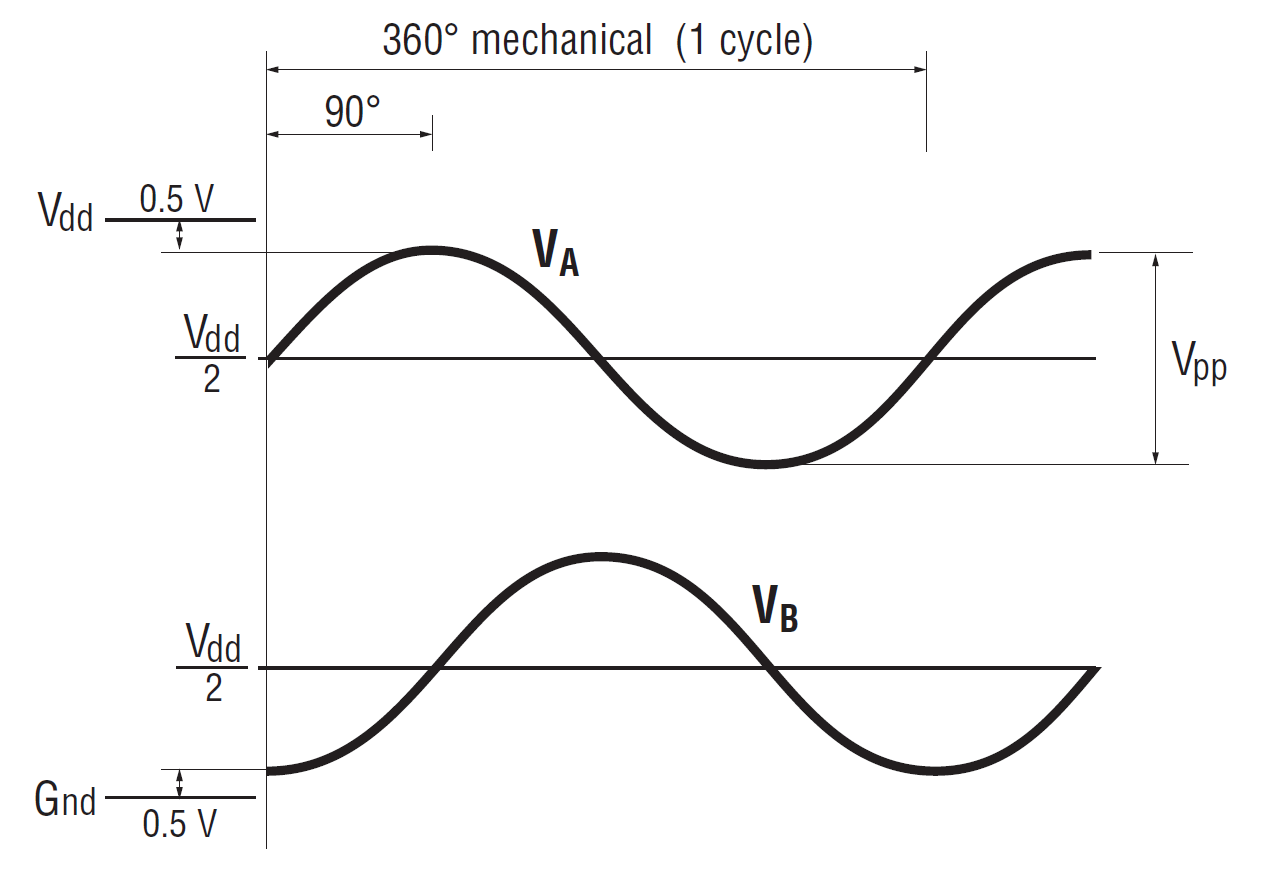
\includegraphics[scale=0.3]{figures/antrieb/SinCos_Sensor.png}
		\caption{Ausgabe eines Sinus/Cosinus-Sensors\cite{Manual}}
	\end{center}
\end{figure}



\newpage

\section{Curtis Controller}
\subsection{Allgemeines}
Der Curtis Controller ermöglicht eine genaue, zuverlässige und hocheffiziente Regelung von Drehzahl und Drehmoment bei Wechselstrom-Induktionsmotoren (ACIM) und Permanentmagnet-Synchronmotoren (SPM). Dieser Motorcontroller verfügt über zwei unabhängige Microprozessoren, um gleichzeitig eine außergewöhnliche Leistungsfähigkeit und funktionale Sicherheit gewährleisten zu können. 

Der primäre Mikroprozessor führt eine fortschrittliche feldorientierte AC-Motorregelung durch, ebenso beinhaltet er einen weiteren integrierten Logik-Prozessor für eine zeitgleiche Operation durch die VCL-Software. Der zweite Mikroprozessor überwacht kontinuierlich den Betrieb des Gesamtsystems. Er misst Eingänge und kontrolliert die zugehörigen Ergebnisse, weiteres überprüft er kritische Zeitpunkte und Operationen. 

Die Vehicle-Control-Language (VCL) ist eine  innovative Programmiersprache, welche von Curtis entwickelt wurde. Sehr viele einzigartige Funktionen sind in dieser Programmiersprache enthalten, weiteres können bei Bedarf selbst Funktionen erstellt und konfiguriert werden. VCL eröffnet neue Möglichkeiten der Anpassung, sodass bestimmte fahrzeugspezifische Anwendungen schnell und einfach in der Motorsteuerung selbst erstellt werden können, um den Einbau von zusätzlichen Steuer-Modulen verhindern zu können.

Für die umfassende Einsatzmöglichkeit dieses Controllers sind ebenfalls sehr wichtige Kommunikationsmöglichkeit über den CAN-Bus gegeben. Ein- und Ausgänge können im gesamten System geteilt und optimal gemeinsam genutzt werden, wodurch die Verkabelung minimiert und zusätzliche Applikationsmöglichkeiten erstellt werden können, die häufig die Kosten des Gesamtsystems senken.

Dieser Motorcontroller ist eine ideale Lösung für Motorantriebe in der Anwendung für Elektrofahrzeuge, Hebevorrichtungen und Doppelmotorantriebe\footnote{vgl. \cite{Manual}, S. 1.}.
\\[10mm]
\begin{figure}[H]
	\begin{center}
		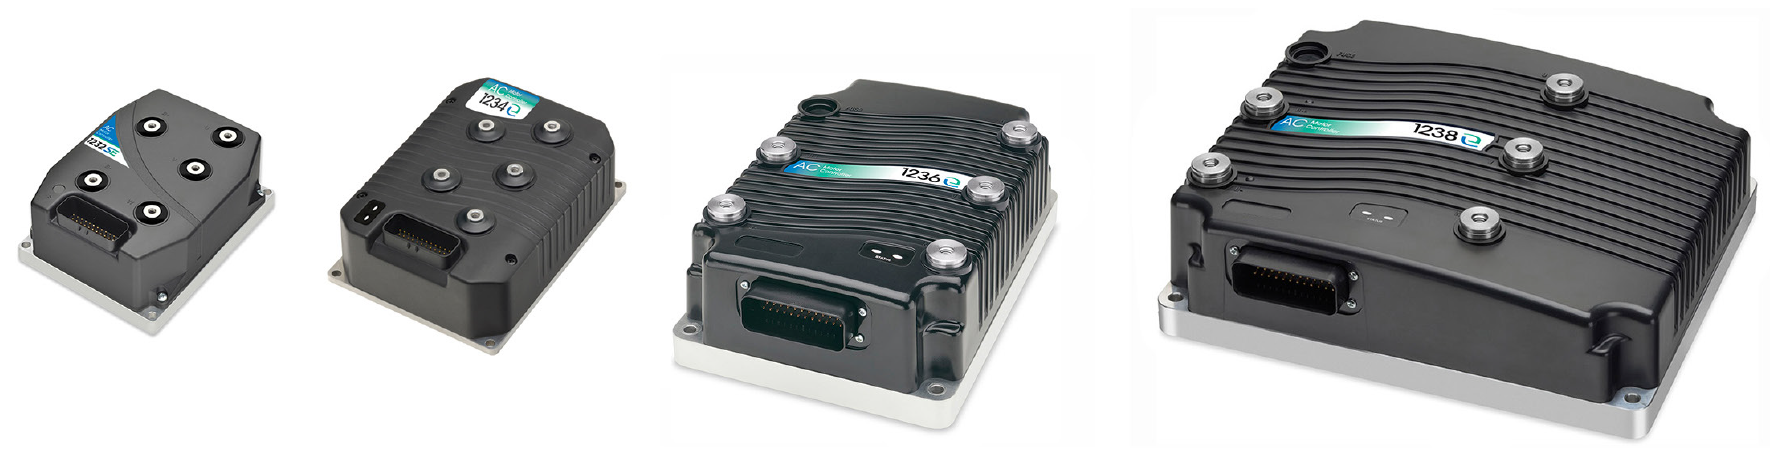
\includegraphics[width=\textwidth]{figures/antrieb/Curtis_Bauformen.png}
		\caption{Übersicht der häufigsten Bauformen eines Curtis Controllers\cite{Manual}}
	\end{center}
\end{figure}



\newpage
 
\subsection{Feldorientierte Regelung}
Die herkömmliche Technik zur Regelung von PSM wird als Sechsstufen- oder Trapezsteuerung bezeichnet. Dabei wir der Stator in einem sechsstufigen Prozess angesteuert, der Schwankungen des erzeugten Drehmoments hervorruft. Jedes Wicklungspaar wird einzeln erregt, bis der Rotor die nächste Position erreicht, dann wird der Motor zum nächsten Schritt kommutiert. Skalare Techniken sind jedoch für Anwendungen mit dynamisch wechselnden Lasten nicht präzise genug. Durch den Einsatz der feldorientierten Regelung lässt sich die Präzision, Effizients und Lebensdauer des Antriebs erheblich steigern, weiteres lassen sich bei hohen und niedrigen Drehzahlen leistungsstarke Drehmomentregelungen realisieren\footnote{vgl. \cite{Feldorientierte-Regelung}}.

Die feldorientierte Regelung (auch Vektorregelung gennant) ist ein sinusförmiges Kommutierungsverfahren. Der Motorcontroller hat die Aufgabe die Statorströme zu berechnen, um den Rotor basierend auf der Stromrückkoppelung des Motors ansteuern zu können. Abgeleitet von der Raumzeigerdarstellung für Wechselspannungen und -strömen und deren bezug zueinander wird ein rotierendes Koordinatensystem mit den Größen Drehmoment und magnetische Flussdichte als Achsen erstellt. Das Verfahren wandelt die Statorströme über dieses Koordinatensystem in magnetische Flussdichte und Drehmoment erzeugende Komponenten um. Zudem regelt es die Statorströme über einen PID-Regler und wandelt sie dann in drei Spannungswerte zurück, aus denen wiederum der PWM-Ausgang erstellt wird. Dieser ist dann auch für das sinusförmige Kommutierungssignal verantwortlich\footnote{vgl. \cite{Feldorientierte-Antriebssteuerung}}.
\\[7mm]
\begin{figure}[H]
	\begin{center}
		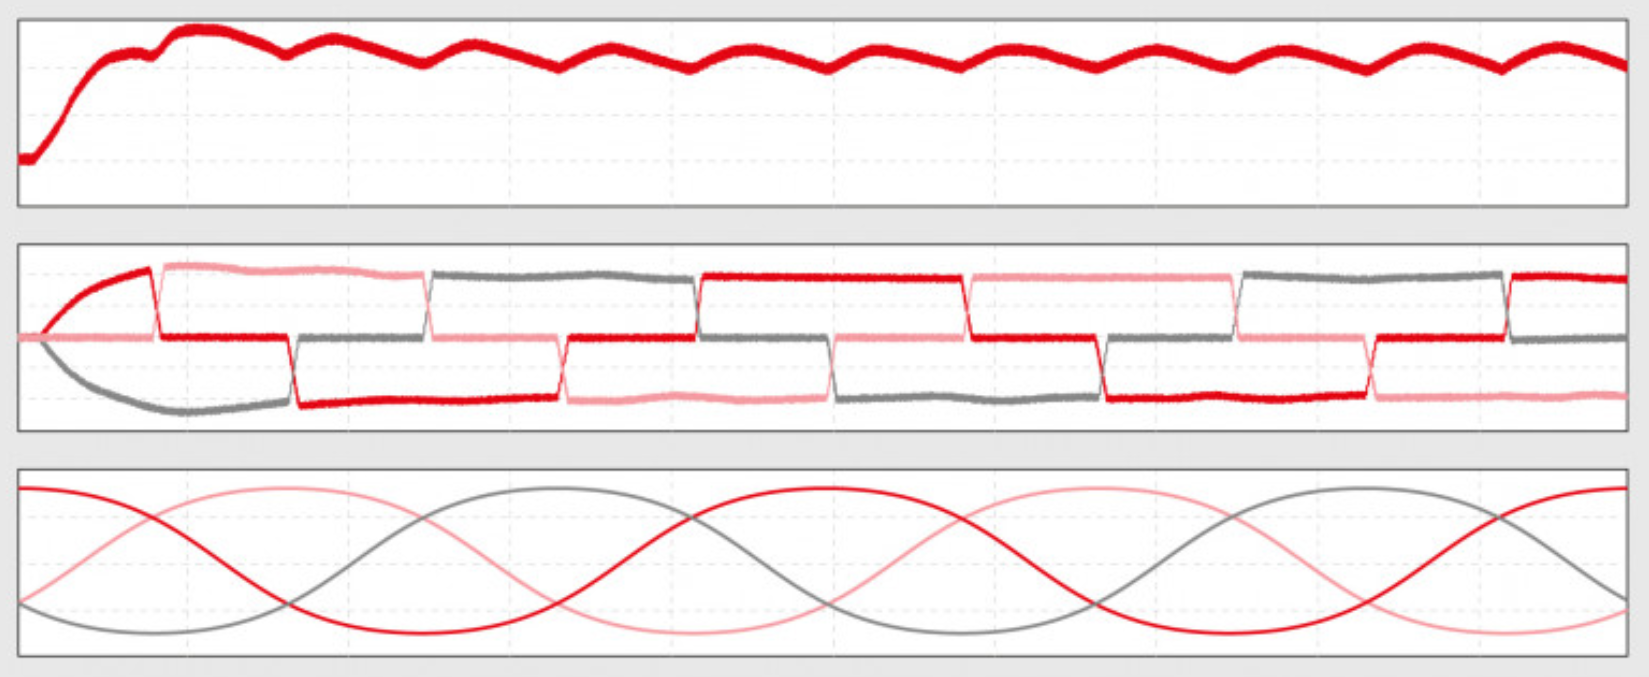
\includegraphics[width=0.9\textwidth]{figures/antrieb/Kommutierung_Trapezsteuerung.png}
		\caption{Kommutierung mittels Trapezsteuerung\cite{Feldorientierte-Antriebssteuerung}}
	\end{center}
\end{figure}

\begin{figure}[H]
	\begin{center}
		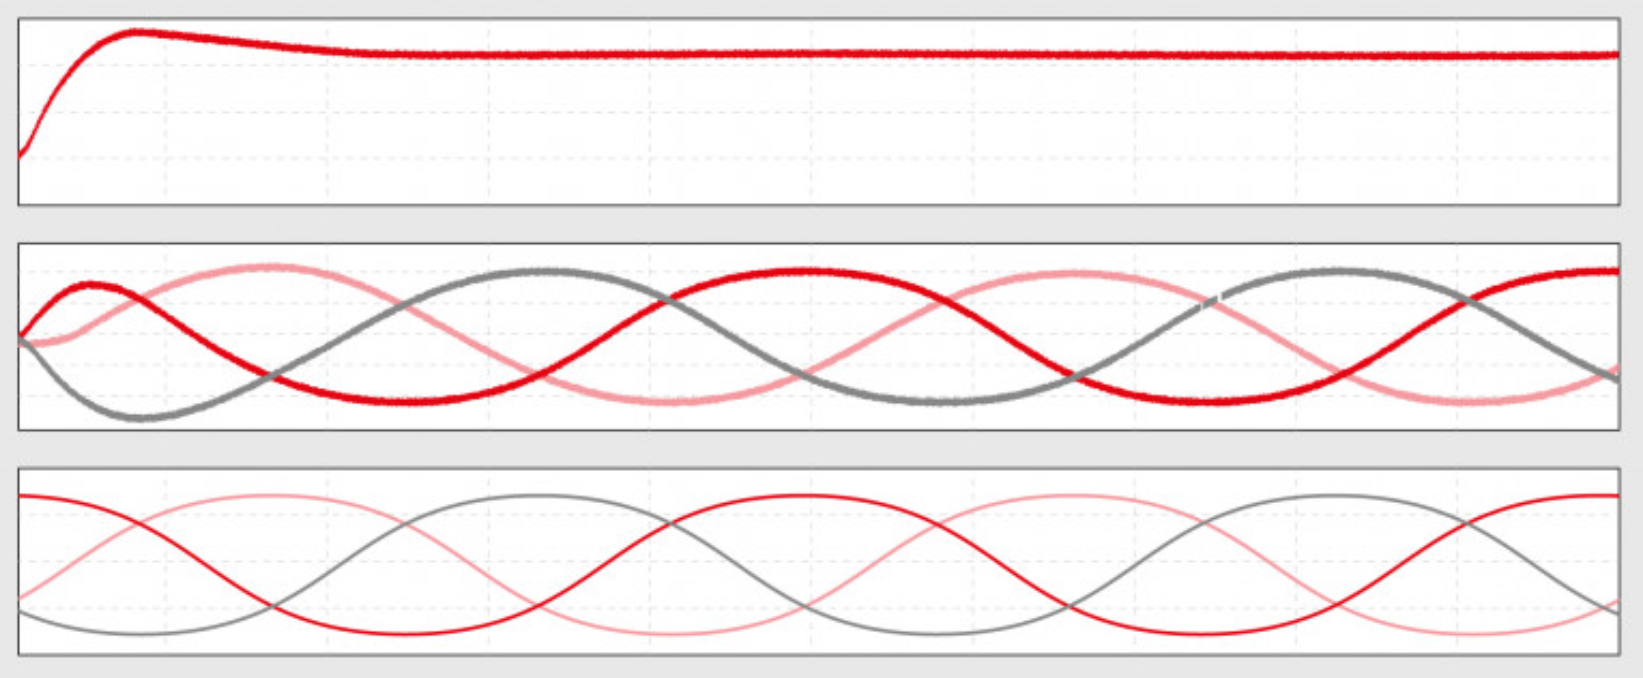
\includegraphics[width=0.9\textwidth]{figures/antrieb/Kommutierung_Vektorregelung.png}
		\caption{Kommutierung mittels Vektorregelung\cite{Feldorientierte-Antriebssteuerung}}
	\end{center}
\end{figure}

%https://www.digikey.de/de/articles/field-oriented-control-of-small-dc-motors-put-drones-on-a-rising-flight-path
%https://www.all-electronics.de/foc-mcu-antriebssteuerung/

\newpage



\section{Der Regler}
\subsection{Einleitung}
Regelungen sind ein Bestandteil unseres Lebens und das nicht nur seit Erfindung der Dampfmaschine.

Allein schon der aufrechte Gang funktioniert nur mit Regelung. Dabei wirken die Sinne als Sensoren, das Gehirn als Regler und die Muskeln als Aktoren. Weitere Regelungen in unserem Körper sind z.B. die Konstanthaltung der Körpertemperatur, der Blutdruck, die Anpassung der Pupille auf Helligkeitsänderungen usw.

Der Begriff Regelung ist zu unterscheiden von dem im allgemeinen Sprachgebrauch oft synonym gebrauchten Begriff der Steuerung. Das Steuern ist ein rein vorwärts gerichteter Prozess ohne Rückkopplung. Die Ausgangsgröße wird dabei nicht überwacht und kann sich durch Störungen von außen verändern. Ein Beispiel ist die Steuerung eines Elektromotors mit einer einstellbaren Spannung. Durch Laständerungen wird sich die Drehzahl des Motors ändern. Soll nun die Drehzahl konstant gehalten werden, bedarf es einer Rückkopplung, um über die Spannung die Drehzahl anzupassen. Diese Rückkopplung ist das Kennzeichen einer Regelung.

Das Regeln ist ein Vorgang, bei dem die Ausgangsgröße, im Beispiel die Drehzahl, fortlaufend überwacht wird und bei Abweichung über die Stellgröße, im Beispiel die Spannung, korrigiert wird. Der sich dabei ergebende Wirkungsablauf findet in einem geschlossenen Kreis, dem Regelkreis, statt.
\vspace{5mm}

\subsection{Der Regelkreis}
Das Prinzip einer Regelung ist das fortlaufende Messen – Vergleichen – Stellen.
\\[5mm]

\begin{itemize}
	\item \textbf{Messen}
	\\[1mm] Die Regelgröße wird mittels Sensoren gemessen.
	\medskip
	\item \textbf{Vergleichen}
	\\[1mm] Der Wert der Regelgröße wird mit dem Sollwert verglichen. Die Differenz ist die Regelabweichung.
	\medskip
	\item \textbf{Stellen}
	\\[1mm] Aus der Regelabweichung wird unter Berücksichtigung der dynamischen Eigenschaften der Regelstrecke die Stellgröße bestimmt.
\end{itemize}
\vspace{3mm}

Ein Regelkreis dient dazu, eine vorgegebene physikalische Größe, die Regelgröße, auf einen gewünschten Wert (Sollwert) zu bringen und dort zu halten, unabhängig von eventuell auftretenden Störungen. Um die Regelungsaufgabe zu erfüllen, muss der Augenblickswert der Regelgröße – der Istwert – gemessen und mit dem Sollwert verglichen werden. Auftretende Abweichungen müssen in geeigneter Art und Weise nachgestellt werden.

Um nun diese Aufgabe technisch zu lösen, gibt es die Regelungstechnik. Sie baut im wesentlichen auf die mathematische Beschreibung und Modellbildung des Systems Regelkreis. Zur Modellierung, Beschreibung und Simulation werden Blockschaltbilder mit diskreten Signalgliedern verwendet\footnote{vgl. \cite{Regelungstechnik}}.
	
\newpage

Ein Regelkreis besteht entsprechend des vereinfachten Blockschaltbildes, wie es oft in der Regelungstechnik verwendet wird, aus den Hauptteilen Regler und Regelstrecke:
\\[5mm]

\begin{itemize}
	\item \textbf{Regler G$_R$}
	\\[1mm] Um die Regelabweichung zu minimieren müssen Korrekturmaßnahmen ergriffen werden.
	\medskip
	\item \textbf{Regelstrecke G$_S$}
	\\[1mm] Das zu regelnde System \medskip
	\item \textbf{Führungsgröße w (Sollwert)}
	\\[1mm] Vorgegebener Wert, auf dem die Regelgröße durch die Regelung gehalten werden soll. \medskip
	\item \textbf{Regelgröße x (Istwert)}
	\\[1mm] Die Ausgangsgröße der Regelstrecke wird für den Vergleich mit dem Sollwert bzw. zur Berechnung der Regelabweichung rückgekoppelt. \medskip
	\item \textbf{Regelabweichung e}
	\\[1mm] Differenz zwischen Führungsgröße und Regelgröße e = w – x, bildet die eigentliche Eingangsgröße des Reglers. \medskip
	\item \textbf{Stellgröße y}
	\\[1mm] Die Ausgangsgröße des Reglers wird vom zu regelnden System beeinflusst. \medskip
	\item \textbf{Störgröße z}
	\\[1mm] Es können unvorhersehbare Störgrößen auftreten, die ebenfalls ausgeregelt werden müssen.
\end{itemize}

\vspace{7mm}
\begin{figure}[H]
	\begin{center}
		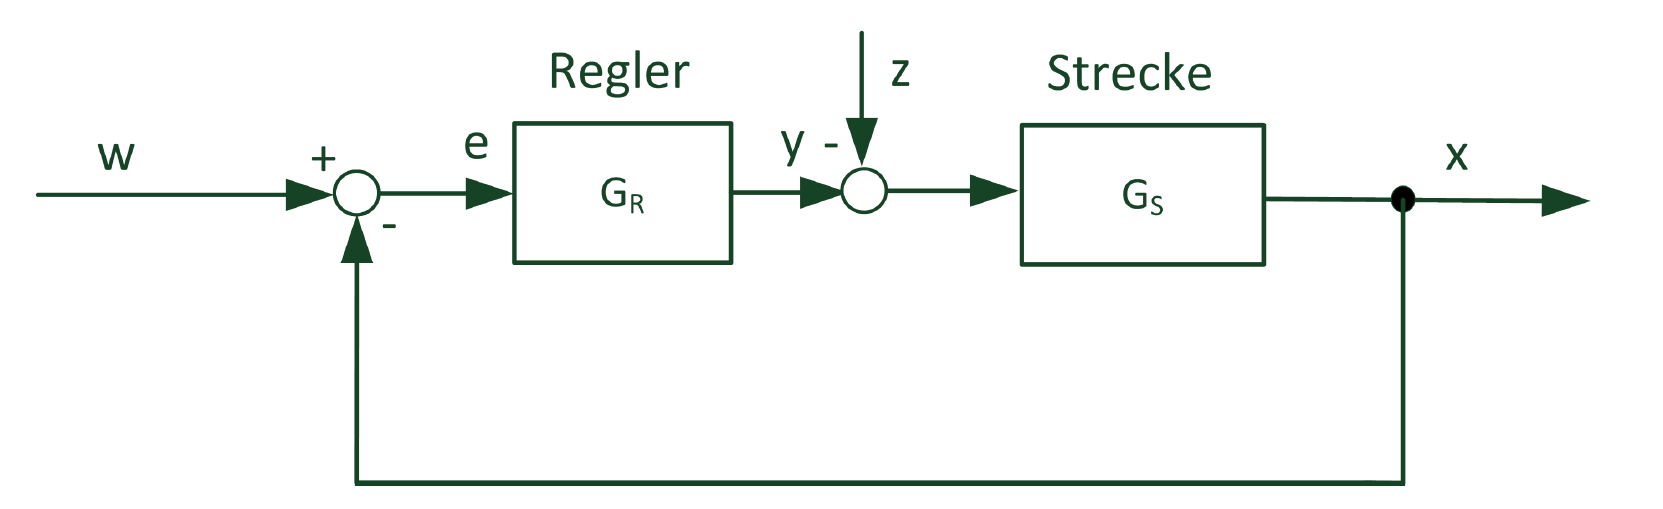
\includegraphics[width=\textwidth]{figures/antrieb/Regelkreis_Grundaufbau.png}
		\caption{Das Blockschaltbild eines allgemeinen Regelkreises\cite{AUT5}}
	\end{center}
\end{figure}

\newpage

\subsection{Der PID-Regler}
Der PID-Regler vereinigt die guten Eigenschaften der anderen klassischen Regler. Der PID-Regler ist genau und sehr schnell, in den meisten Anwendungen kommt deshalb dieser Regler zum Einsatz. Vorab sollte man jedoch überprüfen, ob ein einfacherer bzw. billigerer Regler für die Realisierung der gewünschten Anwendung ebenfalls ausreicht.
\\[5mm]
Der PID-Regler besteht grundlegend aus drei einzelnen Reglern, die mit einander kombiniert werden:
\\[5mm]
\textbf{P-Anteil}\\[1mm]
Der proportionalwirkende Regler multipliziert die Regelabweichung mit seinem Verstärkungsfaktor Kp und gibt das Ergebnis unverzögert weiter. Der P-geregelte Kreis ist einfach und mittelschnell im Vergleich zu anderen Regelungen. Das Problem hierbei ist die bleibende Regelabweichung!
\\[4mm]
Reglergleichung: \hspace{5mm} $y(t) = K_P \cdot e(t)$ \hspace{5mm} bzw. \hspace{5mm} G$_R$ = K$_P$
\\[7mm]

\textbf{I-Anteil}\\[1mm]
Der integralwirkende Regler summiert die Regelabweichung über der Zeit auf und multipliziert die Summe (d.h. das Integral) mit dem Faktor Ki. Je länger eine Regelabweichung ansteht, desto größer wird die Stellgröße des I-Reglers. Der I-geregelte Kreis ist langsam im Vergleich zu anderen Regelungen. Er hat aber den Vorteil, dass die Abweichung vollständig eliminiert wird.
\\[4mm]
Reglergleichung: \hspace{5mm} $y(t) = K_I \cdot \int\limits_{0}^{t} e(t) \,dt$ \hspace{5mm} bzw. \hspace{5mm} $G_R = \dfrac{K_I}{s}$
\\[7mm]

\textbf{D-Anteil}\\[1mm]
Der D-Anteil ist ein Differenzierer, der nur in Verbindung mit anderen Reglern eingesetzt wird. Er reagiert nicht auf die Regelabweichung, sondern nur auf deren Änderungsgeschwindigkeit. Je schneller sich das Signal ändert, desto größer ist die Ausgangsgröße, diese wird noch mit Kd multipliziert.

Ein Nachteil aller Regler mit D-Anteil kann die Unruhe im Kreis sein. Ist das Sensorsignal verrauscht, so wird dieses Rauschen durch das Differenzieren weiter verstärkt und wieder in den Kreis hineingegeben. Dadurch wird der Aktor stärker belastet. Solche Probleme können aber durch Anpassung der Regelparameter oder mit dem Hinzufügen eines Filters behoben werden\footnote{vgl. \cite{AUT5}, Kapitel 4}.
\\[4mm]
Reglergleichung: \hspace{7mm} $y(t) = K_D \cdot \dfrac{de(t)}{dt}$\hspace{5mm} bzw. \hspace{5mm} $G_R = K_D \cdot s$

\newpage

Kombiniert man also die drei unterschiedlichen Regler miteinander, so erhält man den sogennanten PID-Regler, dieser vereint die guten Eigenschaften der einzelnen Regler. Der P-Regler ist für die schnelle Korrekturen zuständig, er reagiert ohne Verzögerung auf die Regelabweichung. Der I-Regler überwacht die Regelung des P-Reglers und korrigiert diese über die Zeit, um eventuelle Regelabweichungen auszubessern. Der D-Anteil verstärkt bei schnellen Veränderungen beide Regelkreise, um das Ansprechverhalten zu verbessern\footnote{vgl. \cite{PID-Regler}}.
\\[4mm]
Reglerleichung: \hspace{3mm} $y(t) = K_P \cdot e(t) + K_I \cdot \int\limits_{0}^{t} e(t) \,dt + K_D \cdot \dfrac{de(t)}{dt}$ \hspace{3mm} bzw. \hspace{3mm} $G_R = K_P + \dfrac{K_I}{s} + K_D \cdot s$
\\[5mm]
\begin{figure}[H]
	\begin{center}
		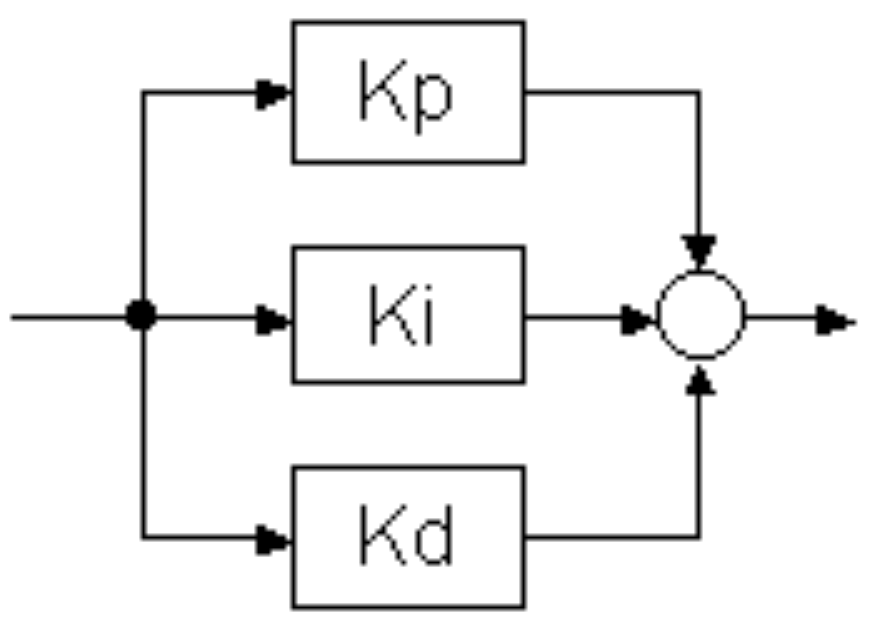
\includegraphics[scale=0.15]{figures/antrieb/PID_Regler.png}
		\caption{Zusammensetzung des PID-Reglers\cite{Regelungstechnik}}
	\end{center}
\end{figure}
\vspace{5mm}
Hier sind für ein besseres Verständnis die Sprungantworten der unterschiedlichen klassischen Reglertypen dargestellt. Der Regelkreis ist geschlossen, ein PT2-Glied bildet die Regelstrecke.
\\[4mm]
\begin{figure}[H]
	\begin{center}
		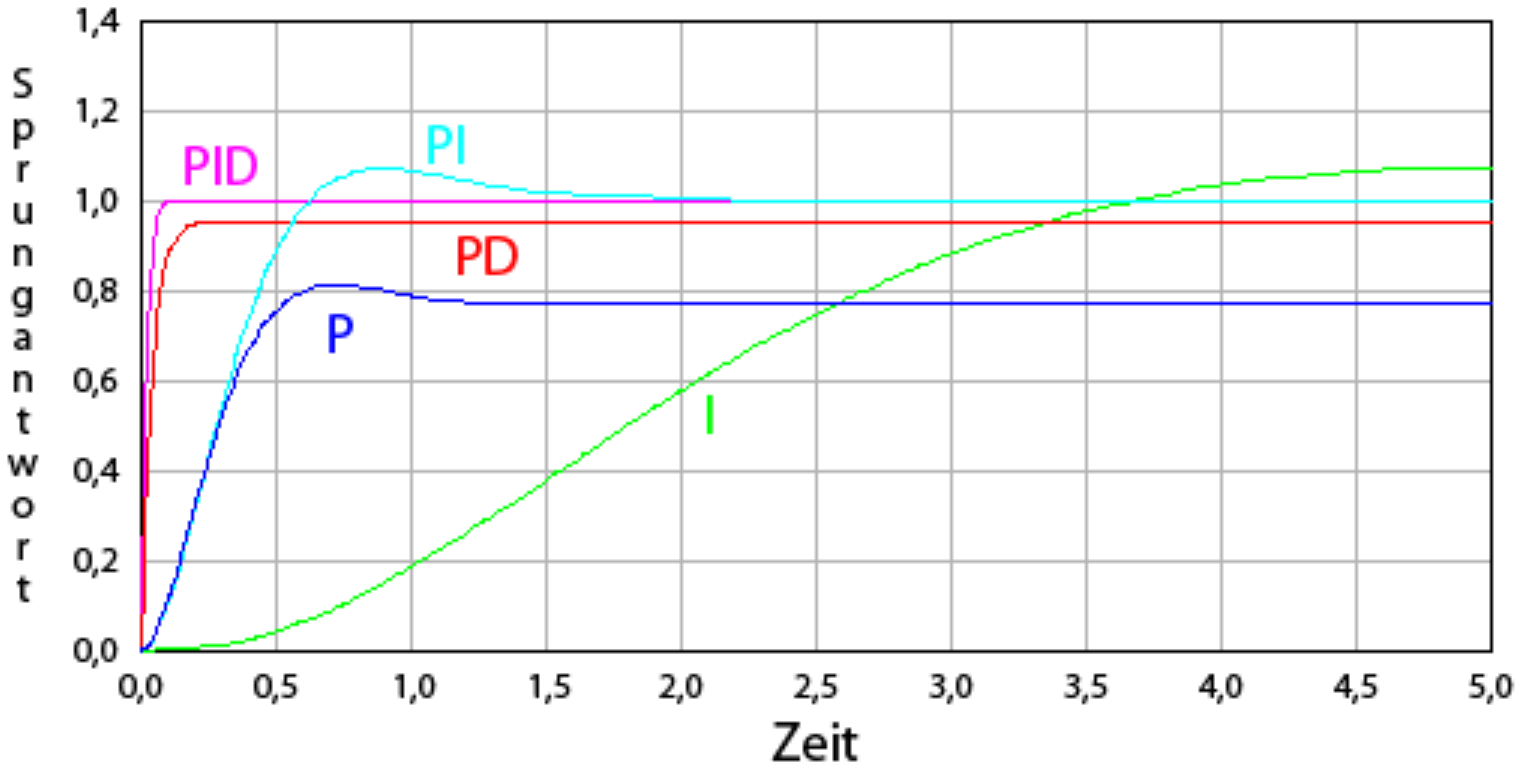
\includegraphics[scale=0.3]{figures/antrieb/Reglertypen.png}
		\caption{Vergleich der verschiedenen Reglertypen\cite{PID-Regler}}
	\end{center}
\end{figure}

%https://rn-wissen.de/wiki/index.php/Regelungstechnik
%http://3digi.wikidot.com/allgemeines-zu-pid-reglern
%AUT5
\newpage

%%%%%%%%%%%%%%%%%%% HCIS

\section{Steuereinheiten}
\section{Bussysteme}
